\usepackage{cleveref}

%!TEX root = ../Thesis.tex
%! Author = PR
%! Date = 27.05.2020


\section{Schnittstellen}

Die Anwendung ist über eine REST-API erreichbar. Alle Antworten sind im JSON-Format. Die Schnittstelle stellt folgende Services bereit:
\begin{itemize}
    \item HTTP Methode: GET
    \item Relativer Pfad: /api/ideas/
    \item Antwort: Array aus Ideen (Proukt-/ Interne Ideen).
    \item Beispielantwort:
    \begin{verbatim}
    [
        {
            "id": 145,
            "title": "Nachmieter für Häuschen in Detmold gesucht!",
            "description": "Och joa ich habe da 'ne Idee",
            "creator": {
            "type": "de.fhdw.geiletypengmbh.digitalerbriefkasten.
            persistance.model.account.User",
            "id": 1,
            "username": "API_USER",
            "roles": [
                {
                    "name": "API_USER"
                }
            ],
            "lastName": "USER",
            "firstName": "API",
            "creationDate": "2020-05-24"
        },
        "creationDate": "2020-05-27",
        "status": "NOT_SUBMITTED",
        "productLine": {
            "id": 2,
            "title": "INTERNAL",
            "specialists": []
        },
        "advantages": [
            {
                "id": 146,
                "description": "Nur"
            },
            {
                "id": 147,
                "description": "Ein"
            },
            {
                "id": 148,
                "description": "Vorteil"
            }
        ],
        "specialist": null,
        "field": {
            "id": 21,
            "title": "Kostensenkung"
        }
        },
        {
            "id": 149,
            "title": "[Reserviert] Nachmieter für Häuschen in Detmold gesucht!",
        "description": "Hmmm.. Naja irgendwas wird es schon werden.",
        "creator": {
            "type": "de.fhdw.geiletypengmbh.digitalerbriefkasten.
            persistance.model.account.User",
            "id": 1,
            "username": "API_USER",
            "roles": [
                {
                    "name": "API_USER"
                }
            ],
            "lastName": "USER",
            "firstName": "API",
            "creationDate": "2020-05-24"
        },
        "creationDate": "2020-05-27",
        "status": "NOT_SUBMITTED",
        "productLine": {
            "id": 3,
            "title": "KFZ",
            "specialists": []
        },
        "advantages": [
            {
                "id": 150,
                "description": ""
            },
            {
                "id": 151,
                "description": ""
            },
            {
                "id": 152,
                "description": ""
            }
        ],
        "specialist": null,
        "targetGroups": [
            {
                "id": 17,
                "title": "Singles"
            }
        ],
        "distributionChannels": [
            {
                "id": 14,
                "title": "Kooperation mit Kreditinstituten"
            }
        ],
        "existsComparable": true
        }
    ]
    \end{verbatim}


\end{itemize}

%
%\begin{figure}[H]
%    \centering
%    \begin{minipage}[H]{1\textwidth}
%        \caption{Grobe Ordnerstruktur}
%        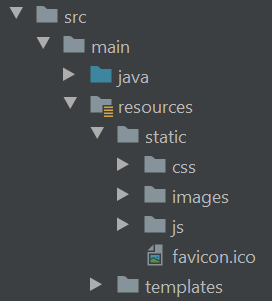
\includegraphics[width=0.5\textwidth]{img/resources-ordner.png}\\
%        \source{Eigene Darstellung}
%        \label{fig:resources-ordner}
%    \end{minipage}
%\end{figure}


